%
% Περάστε στο πακέτο cseuoi-thesis τις κατάλληλες επιλογές για τη διατριβή σας
%
\documentclass[gr,phd]{cseuoi-thesis} % Διδακτορικό (στα Ελληνικά)
%\documentclass[en,msc,systems]{cseuoi-thesis} % Μεταπτυχιακό με εξειδίκευση στα Υπολογιστικά Συστήματα (στα Αγγλικά)
%\documentclass[en,msc,theory]{cseuoi-thesis} % Μεταπτυχιακό με εξειδίκευση στη Θεωρία Επιστήμης Υπολογιστών (στα Αγγλικά)
%\documentclass[en,msc,software]{cseuoi-thesis} % Μεταπτυχιακό με εξειδίκευση στο Λογισμικό (στα Αγγλικά)
%\documentclass[en,msc,scicomp]{cseuoi-thesis} % Μεταπτυχιακό με εξειδίκευση στους Επιστημονικούς Υπολογισμούς (στα Αγγλικά)
%\documentclass[en,msc,techapps]{cseuoi-thesis} % Μεταπτυχιακό με εξειδίκευση στις Τεχνολογίες - Εφαρμογές (στα Αγγλικά)


% 
% Συμπληρώστε τα στοιχεία σας στις παρακάτω εντολές (αφαιρώντας το \colorbox{gray}{})
%
\titleGr{\colorbox{gray}{Τίτλος Διατριβής}}
\titleEn{\colorbox{gray}{Thesis Title}}
\authorGr{\colorbox{gray}{Λεωνίδας Παπαδόπουλος}}
\authorEn{\colorbox{gray}{Leonidas Papadopoulos}}
\arthro{\colorbox{gray}{τον}}
\aitiatiki{\colorbox{gray}{Λεωνίδα Παπαδόπουλο}}
\dateGr{\colorbox{gray}{Φεβρουάριος 2016}}
\dateEn{\colorbox{gray}{February 2016}}
\advisorGr{\colorbox{gray}{Γεώργιος Νικολαΐδης, Επίκουρος Καθηγητής}}
\advisorEn{\colorbox{gray}{Georgios Nikolaidis, Assistant Professor}}


% 
% Για Διδακτορικό συμπληρώστε τις επιτροπές σας (αγνοούνται στο ΜΔΕ)
%
% 3μελής συμβουλευτική επιτροπή
\PHDadvisory{Βασίλειος Βασιλείου}{Επίκ.\ Καθηγητής}%
    {Τμήμα Μηχανικών Η/Υ και Πληροφορικής, Πανεπιστήμιο Ιωαννίνων}
\PHDadvisory{Γεώργιος Γεωργίου}{Αναπλ.\ Καθηγητής}%
    {Τμήμα Μηχανικών Η/Υ και Πληροφορικής, Πανεπιστήμιο Ιωαννίνων}
\PHDadvisory{Δημήτριος Δημητρίου}{Καθηγητής}%
    {Τμήμα Μηχανικών Η/Υ και Πληροφορικής, Πανεπιστήμιο Ιωαννίνων}
% 7μελής εξεταστική επιτροπή
\PHDexaminer{Αντώνιος Αντωνίου}{Αναπλ.\ Καθηγητής}%
    {Τμήμα Μηχανικών Η/Υ και Πληροφορικής, Πανεπιστήμιο Ιωαννίνων}
\PHDexaminer{Βασίλειος Βασιλείου}{Επίκ.\ Καθηγητής}%
    {Τμήμα Μηχανικών Η/Υ και Πληροφορικής, Πανεπιστήμιο Ιωαννίνων}
\PHDexaminer{Γεώργιος Γεωργίου}{Αναπλ.\ Καθηγητής}%
    {Τμήμα Μηχανικών Η/Υ και Πληροφορικής, Πανεπιστήμιο Ιωαννίνων}
\PHDexaminer{Δημήτριος Δημητρίου}{Καθηγητής}%
    {Τμήμα Μηχανικών Η/Υ και Πληροφορικής, Πανεπιστήμιο Ιωαννίνων}
\PHDexaminer{Ιωάννης Ιωάννου}{Αναπλ.\ Καθηγητής}%
    {Τμήμα Μηχανικών Η/Υ και Πληροφορικής, Πανεπιστήμιο Ιωαννίνων}
\PHDexaminer{Νικόλαος Νικολάου}{Αναπλ.\ Καθηγητής}%
    {Τμήμα Μηχανικών Η/Υ και Πληροφορικής, Πανεπιστήμιο Ιωαννίνων}
\PHDexaminer{Πέτρος Πέτρου}{Αναπλ.\ Καθηγητής}%
    {Τμήμα Μηχανικών Η/Υ και Πληροφορικής, Πανεπιστήμιο Ιωαννίνων}

% 
% Εξεταστική επιτροπή για ΜΔΕ
%
\MSCexaminer{Αντώνιος Αντωνίου}{Αναπλ.\ Καθηγητής}%
    {Τμήμα Μηχανικών Η/Υ και Πληροφορικής, Πανεπιστήμιο Ιωαννίνων (Επιβλέπων)}
\MSCexaminer{Βασίλειος Βασιλείου}{Επίκ.\ Καθηγητής}%
    {Τμήμα Μηχανικών Η/Υ και Πληροφορικής, Πανεπιστήμιο Ιωαννίνων}
\MSCexaminer{Γεώργιος Γεωργίου}{Αναπλ.\ Καθηγητής}%
    {Τμήμα Μηχανικών Η/Υ και Πληροφορικής, Πανεπιστήμιο Ιωαννίνων}


% Πακέτο για την εμφάνιση περιθωρίων (χρήσιμο για την εύρεση overfull boxes)
%\usepackage{showframe}

% Πακέτο για τη διατήρηση των floats (εικόνες κ.α.) εντός των ενοτήτων
%\usepackage[section]{placeins}



\begin{document}

% Σελίδες χωρίς αρίθμηση
\pagenumbering{gobble}

% Εκτύπωση της σελίδας τίτλου
\maketitle

% Εκτύπωση της σελίδας με τις επιτροπές
\makecommittees

% Αρχικοποίηση του minitoc
\dominitoc[n]

\chapter*{\cseafierwsi}

Η σελίδα αυτή είναι προαιρετική και περιέχει αφιέρωση σε κάποιο σημαντικό πρόσωπο.

\bigskip

\noindent Προτεινόμενο: 1-2 γραμμές.

\noindent Μέγιστο: 1 σελίδα.
 % Προαιρετικό
\chapter*{\cseeuxaristies}

Η σελίδα αυτή είναι προαιρετική και περιέχει ευχαριστίες σε άτομα που βοήθησαν με οποιονδήποτε τρόπο τον συγγραφέα της διατριβής.

\bigskip

\noindent Προτεινόμενο: 10-15 γραμμές.

\noindent Μέγιστο: 1 σελίδα. % Προαιρετικό


% Σελίδες με αρίθμηση i, ii, iii, iv, ...
\pagenumbering{roman}

% Περιεχόμενα
\pdfbookmark{\contentsname}{contents} % hyperref
\tableofcontents

% Κατάλογος Σχημάτων
\addstarredchapterc{\listfigurename} % minitoc
\listoffigures

% Κατάλογος Πινάκων
\addstarredchapterc{\listtablename} % minitoc
\listoftables

% Κατάλογος Αλγορίθμων
\addstarredchapterc{\listalgorithmname} % minitoc
\listof{algorithm}{\listalgorithmname}

\chapter*{\glossaryname}
% Εισαγωγή του κεφάλαιου στα περιεχόμενα
\addstarredchapter{\glossaryname} %minitoc

Η σελίδα αυτή είναι προαιρετική.
Περιέχει ορισμούς και επεξηγήσεις εννοιών, όρων, συντομεύσεων, και συμβολισμών.
Αν η έκτασή τους είναι μεγαλύτερη από δύο σελίδες τότε πρέπει να πάει στο τέλος της διπλωματικής εργασίας, αμέσως μετά τα παραρτήματα. % Προαιρετικό

% Περίληψη και εκτεταμένη περίληψη
\chapter*{\abstractname}
\addstarredchapter{\abstractname} % minitoc
\makecseabstract


\noindent Η ολοένα και αυξανόμενη ανάγκη για μεγαλύτερη επεξεργαστική ισχύ οδήγησε στη δημιουργία των συστημάτων \textit{μη ομοιόμορφης προσπέλασης μνήμης} (NUMA) τα οποία αποτελούν αρχιτεκτονική εξέλιξη των κοινών \textit{συμμετρικών πολυεπεξεργαστών} (SMPs) και τα οποία είναι εφοδιασμένα με μεγάλους αριθμούς επεξεργαστικών πυρήνων. Τα συστήματα αυτά παρέχουν κοινόχρηστο χώρο διευθύνσεων και συνεπώς επιτρέπουν την ανάπτυξη προγραμμάτων με διαδεδομένες \textit{διεπαφές προγραμματισμού εφαρμογών} (APIs) όπως το OpenMP. Λόγω της πολύπλοκης αρχιτεκτονικής οργάνωσης των συστημάτων NUMA, η επίτευξη των βέλτιστων δυνατών επιδόσεων συνήθως απαιτεί την εκμετάλλευση πληροφοριών που σχετίζονται με την τοπολογία του υποκείμενου συστήματος, δηλαδή με το πώς είναι οργανωμένο το υλικό. Ήδη από την έκδοση 4.0 του OpenMP, άρχισαν να προδιαγράφονται λειτουργίες όπως τα OpenMP places και OpenMP processor binding policies οι οποίες σχετίζονται με την τοπολογία και επιτρέπουν στο χρήστη να ελέγξει τον τρόπο ανάθεσης των νημάτων στα διαθέσιμα επεξεργαστικά στοιχεία. Στα πλαίσια της παρούσας διπλωματικής εργασίας, θα ασχοληθούμε με την υλοποίηση των λειτουργιών OpenMP places και OpenMP processor binding policies, καθώς επίσης θα προσπαθήσουμε να βελτιώσουμε τις υπάρχουσες λειτουργίες συγχρονισμού, όπως οι \textit{κλήσεις φραγής} (barriers), ώστε να λειτουργούν αποδοτικά σε συστήματα NUMA.


\bigskip
\chapter*{\cseextabstract}
\label{ch:ExtendedAbstract}
% Εισαγωγή του κεφάλαιου στα περιεχόμενα
\addstarredchapter{\cseextabstract} % minitoc
% Για την χρήση των \@author, \@date και \@title
\makeatletter

\colorbox{gray}{Όνομα Επώνυμο}.\\
\cseextabstracttype\ \cseextabstractcs, \@date.\\
\cseextabstractdpt\\
\colorbox{gray}{Τίτλος Διατριβής.}\\
\cseextabstractsup: \colorbox{gray}{Όνομα Επώνυμο}.\\
\bigskip

\noindent Εκτεταμένη περίληψη της εργασίας στην αντίθετη
γλώσσα από αυτήν του κειμένου. (Αν το κείμενο είναι στα
Ελληνικά αυτή η σελίδα πρέπει να είναι στα Αγγλικά, αν
το κείμενο είναι στα Αγγλικά τότε και αυτή η σελίδα να
είναι στα Ελληνικά.)

\y\noindent Προτεινόμενο μέγεθος: 2 σελίδες.

\y\noindent Μέγιστο μέγεθος: 4 σελίδες.


% Σελίδες με αρίθμηση 1, 2, 3, 4, ...
\pagenumbering{arabic}

% Εισαγωγή των κεφαλαίων
\chapter{Εισαγωγή}
\label{ch:Introduction}

\section{Η ανάγκη για παράλληλα συστήματα} % Η εξέλιξη των σύγχρονων Η/Υ
\label{sec:The need for parallel systems}
Η βασική ιδέα της οργάνωσης των ηλεκτρονικών υπολογιστών με τη μορφή που αυτοί είναι γνωστοί έως και σήμερα, βασίζεται στην αρχιτεκτονική von Neumann όπως αυτή περιγράφηκε το 1945 από τον ουγγρικής και αμερικανικής καταγωγής μαθηματικό John von Neumann. Βάσει αυτής της περιγραφής, υπάρχει μία μονάδα επεξεργασίας η οποία επικοινωνεί με το τμήμα μνήμης, εκτελώντας εντολές και τροποποιώντας δεδομένα. Ο επεξεργαστής λαμβάνει μία-μία τις εντολές από τη μνήμη και τις εκτελεί προσπελαύνοντας ή/και τροποιοιώντας δεδομένα που βρίσκονται στη μνήμη όταν αυτό καθορίζεται από την εντολή, με αυτό τον κύκλο να επαναλαμβάνεται συνεχώς. Το μοντέλο προγραμματισμού που χρησιμοποιείται στη συγκεκριμένη αρχιτεκτονική είναι γνωστό και ως σειριακό μοντέλο και φαίνεται στο Σχήμα X.

Η εποχή της πληροφορίας που ξεκίνησε στα μέσα του 20\textsuperscript{ού} αιώνα και οδήγησε σε μία οικονομία βασισμένη στην τεχνολογία της πληροφορίας, καθώς και η ολοένα και μεγαλύτερη χρήση των Η/Υ σε κάθε πτυχή της ζωής του ανθρώπου είχαν ως αποτέλεσμα την έναρξη ενός αγώνα ταχύτητας με σκοπό την κατασκευή όλο και πιο γρήγορων υπολογιστών.

Η κλιμάκωση της συχνότητας (frequency scaling) που αφορά την αύξηση της συχνότητας ενός επεξεργαστή με στόχο την επίτευξη μεγαλύτερης επίδοσης στα συστήματα που τον χρησιμοποιούν, αποτέλεσε τον κύριο λόγο αύξησης των επιδόσεων των εμπορικών Η/Υ από τα μέσα του 1980 έως και περίπου τα τέλη του 2004, όταν αυτή η προσπάθεια προσέκρουσε στο τείχος της ισχύος (power wall) όπως φαίνεται στο Σχήμα Χ. Αυτό συνέβει καθώς η αύξηση της συχνότητας οδήγησε στην αύξηση της καταναλισκόμενης ισχύος η οποία με τη σειρά της είχες ως αποτέλεσμα την αύξηση του κόστους λειτουργίας αλλά και την οδήγηση του υλικού στα όριά του με χαρακτηριστικό παράδειγμα την υπερθέρμανσή του.

%Η κλιμάκωση της συχνότητας (frequency scaling) αφορά την αύξηση της συχνότητας ενός επεξεργαστή με στόχο την επίτευξη μεγαλύτερης επίδοσης στα συστήματα που χρησιμοποιούν αυτόν τον επεξεργαστή. Η κλιμάκωση της συχνότητας αποτέλεσε την κινητήριο δύναμη που οδήγησε στην αύξηση των επιδόσεων των εμπορικών Η/Υ από τα μέσα του 1980 έως και περίπου τα τέλη του 2004, μέχρις ότου αυτή η προσπάθεια προσέκρουσε στο τείχος της ισχύος (power wall). Αυτό συνέβει καθώς η αύξηση της συχνότητας οδήγησε στην αύξηση της καταναλισκόμενης ισχύος η οποία με τη σειρά της οδήγησε σε μεγάλη κατανάλωση ρεύματος και υπερθέρμανση του υλικού.

Για να ξεπεραστεί το τείχος της ισχύος, οι κατασκευαστές των επεξεργαστών άρχισαν να ενσωματώνουν παραπάνω του ενός επεξεργαστικούς πυρήνες στο ίδιο ολοκληρωμένο κύκλωμα επεξεργαστή. Η αρχιτεκτονική αυτή βελτίωση είχε ως αποτέλεσμα τη γέννηση των πρώτων πολυπύρηνων επεξεργαστών οι οποία έκαναν δυνατή την ταυτόχρονη εκτέλεση εντολών. Τα συστήματα που περιείχαν πολυπύρηνους επεξεργαστές αποτέλεσαν τα πρώτα εμπορικά μικρού μεγέθους παράλληλα συστήματα.

Στη σημερινή εποχή, τα πολυπύρηνα συστήματα είναι ευρέως διαδεδομένα καθώς απαντώνται από κινητά τηλέφωνα και ενσωματωμένους υπολογιστές χαμηλού κόστους και μεγέθους όσο μια πιστωτική κάρτα τραπέζης, μέχρι και υπολογιστικά συστήματα πολύ υψηλών επιδόσεων που διεξάγουν επιστημονικούς υπολογισμούς.


\section{Κατηγορίες Παράλληλων Συστημάτων}
\label{sec:Parallel System Categories}
Όταν μιλάμε για παράλληλα συστήματα ουσιαστικά αναφερόμαστε σε συστήματα με μία συλλογή από επεξεργαστικές μονάδες που επικοινωνούν και συνεργάζονται για τη λύση ενός προβλήματος. Το πρόβλημα χωρίζεται σε επιμέρους εργασίες οι οποίες με τη σειρά τους ανατίθενται στις επεξεργαστικές μονάδες για εκτέλεση. Παρόλο που η ιδέα των πολλαπλών επεξεργαστικών μονάδων φαίνεται απλή, προκύπτουν ζητήματα τα οποία σχετίζονται πλην άλλων με τον τρόπο:
\begin{itemize}
	\item επικοινωνίας, συγχρονισμού και συντονισμού των επεξεργαστικών μονάδων
	\item διαμοιρασμού των εργασιών και
	\item προγραμματισμού ανάλογα με την οργάνωση του εκάστοτε συστήματος.
\end{itemize}
 
\subsection{Ταξινομία του Flynn}
Μία αρχική κατηγοριοποίηση των παράλληλων συστημάτων μπορεί να γίνει βάσει της ταξινομίας του Flynn και η οποία περιλαμβάνει τις εξής κατηγορίες:
\begin{itemize}
	\item SISD (single-instruction single-data) Σχήμα Χ
	\item SIMD (single-instruction multiple-data) Σχήμα Χ και
	\item MIMD (mutiple-instruction multiple-data) Σχήμα Χ
\end{itemize}

Στην κατηγορία SISD ανήκουν οι κλασικοί σειριακοί υπολογιστές οι οποίοι εκτελούν μία εντολή τη φορά (single-instruction) επάνω σε ένα δεδομένο (single-data). Στην κατηγορία SIMD συναντάμε επίσης υπολογιστές οι οποίοι εκτελούν μία εντολή τη φορά, αλλά μπορούν να την εφαρμόσουν ταυτόχρονα σε πολλαπλά δεδομένα (multiple-data) ώστε να εκμεταλλευτούν την παραλληλία επιπέδου δεδομένων (data-level parallelism). Τέλος, η κατηγορία MIMD θεωρείται ως η κατηγορία των καθαρά παράλληλων υπολογιστών οι οποίοι μπορούν και εκτελούν ταυτόχρονα πολλαπλές εντολές, με κάθε μία να ασχολείται με διαφορετικό δεδομένο.

Όπως θα δούμε στη συνέχεια, οι υπολογιστές MIMD, μπορούν να κατηγοριοποιηθούν περαιτέρω βάσει του πώς είναι οργανωμένη η μνήμη τους.

\subsection{Ταξινόμηση βάσει της οργάνωσης της μνήμης}
Η ταξινόμηση των παράλληλων υπολογιστών σχετικά με το πώς είναι οργανωμένη η μνήμη μπορεί να γίνει είτε βάσει της φυσικής οργάνωσης της μνήμης είτε βάσει της εικόνας/άποψης που έχει ο προγραμματιστής για αυτή.

Σχετικά με την πρώτη κατηγοριοποίηση, οι παράλληλοι υπολογιστές διακρίνονται σε υπολογιστές με (φυσικά) κοινόχρηστη μνήμη (γνωστοί και ως πολυεπεξεργαστές) και σε υπολογιστές με (φυσικά) κατανεμημένη μνήμη.

Όσον αφορά την εικόνα που έχει ο προγραμματιστής για την οργάνωση της μνήμης, οι υπολογιστές μπορούν να διαχωριστούν σε υπολογιστές με κοινόχρηστο και σε υπολογιστές με κατανεμημένο χώρο διευθύνσεων. Αξίζει να σημειωθεί ότι η εικόνα από προγραμματιστική άποψη δεν ταυτίζεται απαραίτητα με την φυσική οργάνωση της μνήμης καθώς με χρήση ειδικού λογισμικού ένα σύστημα με φυσικά κατανεμημένη μνήμη μπορεί να παρέχει κοινόχρηστο χώρο διευθύνσεων.


\subsubsection{Συστήματα κοινόχρηστης μνήμης}
Τα συστήματα κοινόχρηστης μνήμης (SMM - Shared Memory Machines *bib*) αποτελούνται από επεξεργαστές, κοινόχρηστη μνήμη (γνωστή και ως καθολική) η οποία είναι καθολικά προσβάσιμη από όλους τους επεξεργαστές και ένα δίκτυο διασύνδεσης για την επικοινωνία των επεξεργαστών με τη μνήμη. Από άποψη φυσικής οργάνωσης, η μνήμη μπορεί να αποτελείται από περισσότερα του ενός τμήματα/μέρη (modules) τα οποία όμως παρέχουν έναν κοινόχρηστο χώρο διευθύνσεων που είναι προσβάσιμος από όλους τους επεξεργαστές. Οι επεξεργαστές επικοινωνούν, συνεργάζονται και ανταλλάσσουν δεδομένα διαβάζοντας ή γράφοντας σε κοινόχρηστες μεταβλητές που βρίσκονται αποθηκευμένες στη μνήμη.

Το δίκτυο διασύνδεσης επεξεργαστών-μνήμης μπορεί να είναι ένας απλός δίαυλος (bus), ένα διακοπτικό δίκτυο (π.χ. crossbar) ή κάποιο δίκτυο πολλαπλών επιπέδων (π.χ. Δίκτυο Δέλτα). Στην περίπτωση που το δίκτυο διασύνδεσης είναι δίαυλος, τότε αναφερόμαστε σε αυτά τα συστήματα ως Συμμετρικοί Πολυεπεξεργαστές (SMPs - Symmetric Multiprocessors). Οι Συμμετρικοί Πολεπεξεργαστές διαθέτουν μία κοινόχρηστη μνήμη η οποία απέχει εξίσου από όλους τους επεξεργαστές και συνεπώς χαρακτηρίζονται ως συστήματα ομοιόμορφης προσπέλασης μνήμης (UMA - Uniform Memory Access). Όπως είναι φυσικό, αν οι επεξεργαστές είναι πολυπύρηνοι και διαθέτουν ιεραρχία από πολύ μικρές αλλά ταυτόχρονα πολύ γρήγορες μνήμες γνωστές ως κρυφές μνήμες (caches), τότε ο κάθε πολυπύρηνος επεξεργαστής αποτελεί ένα σύστημα SMP καθώς η πρόσβαση στην κρυφή μνήμη είναι πιο γρήγορη από την πρόσβαση στην κύρια μνήμη μέσω του διαύλου.

Επειδή το εύρος ζώνης (bandwidth) του διαύλου είναι σταθερό ανεξάρτητα από το πλήθος των επεξεργαστών που είναι συνδεδεμένοι σε αυτόν, όσο πιο πολλοί επεξεργαστές είναι συνδεδεμένοι, τόσο πιο πολύ υποβαθμίζεται η αποδοτικότητα του δικτύου λόγω των συγγρούσεων πρόσβασης στο κοινό μέσο και συνεπώς τόσο περισσότερο καθυστερεί η εξυπηρέτηση προσπελάσεων στη μνήμη. Για την αποδοτική υποστήριξη μεγαλύτερου αριθμού επεξεργαστών καταφεύγουμε στη χρήση κρυφής μνήμης ή άλλου τύπου δίκτυου διασύνδεσης.

Παράλληλα συστήματα μεγαλύτερου μεγέθους μπορούν να υλοποιηθούν χρησιμοποιώντας Συμμετρικούς Πολυεπεξεργαστές ως κόμβους ενός δικτύου διασύνδεσης (Σχήμα Χ). Σε αυτά τα συστήματα καθίσταται δυνατή η παροχή ενός κοινόχρηστου χώρου διευθύνσεων με χρήση κατάλληλων πρωτοκόλλων συνοχής τα οποία αποκρύπτουν από τον χρήστη του συστήματος την κατανεμημένη οργάνωση της φυσικής μνήμης. Η αρχιτεκτονική που μόλις περιγράφηκε είναι γνωστή και ως κατανεμημένη κοινόχρηστη μνήμη (DSM - Distrubuted Shared Memory), ενώ τα συστήματα αυτά ονομάζονται συστήματα ανομοιόμορφης προσπέλασης μνήμης (NUMA - Non-Uniform Memory Access). Σε περίπτωση ύπαρξης ιεραρχίας κρυφών μνημών στους κόμβους (Σχήμα Χ), χρειάζεται η χρήση ενός πρωτοκόλλου συνοχής κρυφής μνήμης (cache coherence protocol) το οποίο θα εξασφαλίζει ανά πάσα στιγμή ότι οποιαδήποτε προσπέλαση μνήμης θα επιστρέφει την πιο πρόσφατη τιμή. Τέτοια συστήματα είναι γνωστά ως cc-NUMA (Cache coherent NUMA).

\subsubsection{Συστήματα κατανεμημένης μνήμης}
Τα συστήματα κατανεμημένης μνήμης (DMM - Distributed Memory Machines) αποτελούνται από επεξεργαστικά στοιχεία (γνωστά και ως κόμβοι) και από ένα δίκτυο διασύνδεσης το οποίο επιτρέπει την επικοινωνία μεταξύ των κόμβων (Σχήμα Χ) *ref*. Κάθε κόμβος περιέχει επεξεργαστή, τοπική μνήμη και ίσως περιφερειακές συσκευές. Η τοπική μνήμη κάθε κόμβου είναι απευθείας προσβάσιμη μόνο από τον επεξεργαστή του ίδιου κόμβου, ενώ όταν κάποιος επεξεργαστής χρειάζεται να προσπελάσει την τοπική μνήμη που βρίσκεται σε κάποιον άλλο κόμβο, αυτό επιτυγχάνεται με τη μεταβίβαση μηνυμάτων μέσω του δικτύου διασύνδεσης. 

Συλλογές υπολογιστών που είναι συνδεδεμένοι μέσω δικτύου διασύνδεσης αφιερωμένου αποκλειστικά στη μεταξύ τους επικοινωνία ονομάζονται συστάδες (clusters). Οι συστάδες υπολογιστών χρησιμοποιούνται ευρέως λόγω της διαθεσιμότητας δικτύων διασύνδεσης υψηλών επιδόσεων όπως το Switched Gigabit Ethernet, το Infiniband, το Myriret κ.ά. Πολλαπλές συστάδες υπολογιστών μπορούν να διασυνδεθούν μεταξύ τους και να δημιουργήσουν συστήματα πλέγματος (grids).

Το πλήθος των κόμβων και αντίστοιχα το πλήθος των επεξεργαστών στα συστήματα κατανεμημένης μνήμης μπορεί να φτάσει τις δεκάδες χιλιάδες, σε αντίθεση με τα συστήματα κοινόχρησης μνήμης όπου το πλήθος των επεξεργαστών περιορίζεται σε μερικές δεκάδες. Προφανώς, η ικανότητα κλιμάκωσης των κατανεμημένων συστημάτων εξαρτάται από την σωστή επιλογής της τοπολογίας του δικτύου διασύνδεσης.


\section{Προγραμματισμός Παράλληλων Συστημάτων}

\subsection{Συστήματα κοινόχρηστης μνήμης}
Ο προγραμματισμός των συστημάτων κοινόχρηστης μνήμης συνήθως βασίζεται στη χρήση νημάτων, δηλαδή ξεχωριστές ακολουθίες ελέγχου (στοίβα + μετρητής προγράμματος) που μοιράζονται δεδομένα με τα υπόλοιπα άλλα νήματα μέσω κοινόχρηστου χώρου διευθύνσεων. Η ύπαρξη κοινόχρηστων δεδομένων εγείρει ζητήματα όπως αυτό της ταυτόχρονης προσπέλασής τους από διαφορετικά νήματα, καθώς κάτι τέτοιο θα μπορούσε να οδηγήσει σε συνθήκες ανταγωνισμού (race conditions). Όταν υπάρχουν συνθήκες ανταγωνισμού, το τελικό αποτέλεσμα των ταυτόχρονων προσπελάσεων μνήμης εξαρτάται από τις σχετικές ταχύτητες εκτέλεσεις των νημάτων. Για την αποφυγή συνθηκών ανταγωνισμού και την εξασφάλιση της ακεραιότητας των δεδομένων χρησιμοποιείται ο αμοιβαίος αποκλεισμός (mutual exclusion), βάσει του οποίου μόνο ένα νήμα κάθε φορά μπορεί να εκτελεί εντολές που τροποποιούν κοινόχρηστες μεταβλητές.

Η πιο διαδεδομένη βιβλιοθήκη νημάτων και μοντέλο εκτέλεσης είναι αυτό των POSIX threads (pthreads) το οποίο παρέχει κλήσεις διαχείρισης (π.χ. δημιουργία, τερματισμό) νημάτων, κλειδαριές (mutexes), μεταβλητές συνθήκης (condition variables) και κλήσεις συγχρονισμού νημάτων όπως για παράδειγμα κλήσεις φραγής (barriers). Ο προγραμματιστής έχει την πλήρη ευθύνη για τη δημιουργία των νημάτων, την ανάθεση εργασιών σε αυτά, προεραιτικά την αντιστοίχηση των νημάτων σε επεξεργαστές, πιθανώς την συλλογή των επιμέρους αποτελεσμάτων και την σύνθεση του τελικού αποτελέσματος από αυτά, καθώς και τον τερματισμό τους. Επιπλέον, είναι υπεύθυνος για τον συγχρονισμό των νημάτων και την αποφυγή συνθηκών ανταγωνισμού με χρήση κατάλληλων προγραμματιστικών δομών.

Για τη διευκόλυνση του προγραμματισμού, μπορούν να χρησιμοποιηθούν εργαλεία πιο υψηλού επιπέδου όπως το OpenMP (Open Multi-Processing). Το OpenMP είναι μία διεπαφή προγραμματισμού εφαρμογών (API - Application Programming Interface) η οποία αποτελείται από οδηγίες (directives) προς τον μεταφραστή, ρουτίνες βιβλιοθήκης και μεταβλητές περιβάλλοντος (environment variables) και συντελεί στην συγγραφή πολυνηματικού κώδικα για συστήματα κοινόχρηστης μνήμης. Πολύ σημαντικό είναι το γεγονός ότι το OpenMP δίνει τη δυνατότητα παραλληλοποίησης του υπάρχοντα σειριακού κώδικα χωρίς την τροποποίησή του, παρά μόνο με την προσθήκη των ειδικών οδηγιών οι οποίες μπορούν να αγνοηθούν σε περίπτωση που δεν υποστηρίζονται από κάποιο μεταφραστή. Επίσης, η διαχείριση των νημάτων γίνεται αυτόματα, ενώ όλα τα υπόλοιπα ζητήματα που σχετίζονται με τον συγχρονισμό, ανάθεση εργασιών κλπ απλοποιούνται σε μεγάλο βαθμό. Η απλότητα του OpenMP αλλά και όλες οι διευκολύνσεις που προσφέρει, το κάνουν να βρίσκεται στην κορυφή των προτιμήσεων για προγραμματισμό συστημάτων κοινόχρηστης μνήμης, αφού μπορεί να χρησιμοποιηθεί ακόμα και από προγραμματιστές χωρίς ιδιαίτερη εμπειρία ή γνώσεις σχετικά με την παράλληλη επεξεργασία. Περισσότερα για το πρότυπο OpenMP θα ειπωθούν στο Κεφάλαιο Χ.


\subsection{Συστήματα κατανεμημένης μνήμης}
Ο προγραμματισμός των συστημάτων κατανεμημένης μνήμης συνήθως βασίζεται στη μεταβίβαση μηνυμάτων μεταξύ αυτόνομων διεργασιών (προγράμματα υπό εκτέλεση) οι οποίες βρίσκονται σε διαφορετικούς κόμβους και δεν μοιράζονται κοινόχρηστες μεταβλητές, αλλά πραγματοποιούν μεταξύ τους αποστολή και λήψη μηνυμάτων. Η μη ύπαρξη κοινόχρηστων δεδομένων εξαλείφει την ανάγκη για αμοιβαίο αποκλεισμό αλλά ταυτόχρονα δυσκολεύει τον συγχρονισμό μεταξύ των διεργασιών. Ο προγραμματιστής είναι υπεύθυνος να καθορίσει πότε σταματούν οι υπολογισμοί και πότε ξεκινούν οι επικοινωνίες, το περιεχόμενο, τον αποστολέα και τους παραλήπτες των μηνυμάτων, καθώς και να αποφασίσει τον τύπο της επικοινωνίας που θα χρησιμοποιήσει (σύγχρονη ή ασύγχρονη).

Στις σύγχρονες επικοινωνίες μία διεργασία που θέλει να στείλει (λάβει) δεδομένα μπλοκάρει στην αντίστοιχη κλήση αποστολής (λήψης) μέχρις ότου η διαδικασία παραλήπτης (αποστολέας) παραλάβει (αποστείλει) τα δεδομένα. Ο τρόπος λειτουργίας των σύγχρονων επικοινωνιών τις καθιστά ιδανικές για την επίτευξη συγχρονισμού μεταξύ των διεργασιών. Αντίθετα, στις ασύγχρονες επικοινωνίες, η διεργασία δεν "μπλοκάρει" αλλά συνεχίζει κανονικά την εκτέλεση της.

Λόγω της φύσης του μοντέλου μεταβίβασης μηνυμάτων, ο προγραμματιστής θα πρέπει να δώσει προσοχή στο πώς θα ελαχιστοποιήσει την επικοινωνία μεταξύ διαφορετικών κόμβων, καθώς η προσπέλαση της τοπικής μνήμης κάθε κόμβου είναι πολύ πιο γρήγορη απ' ότι η προσπέλαση της μνήμης άλλων κόμβων. Γι' αυτό το λόγο πρέπει να σχεδιαστεί με σύνεση ο διαμοιρασμός των δεδομένων ανάμεσα στους κόμβους, καθώς και η ανάθεση φόρτου σε κάθε διεργασία ώστε εκτός από την αποφυγή καθυστερήσεων σε απομακρυσμένες προσπελάσεις, να αποφευχθεί και συμφόρηση του δίκτυου.

Δημοφιλές πρότυπο μεταβίβασης μηνυμάτων αποτελεί το MPI (Message Passing Interface) με τις δύο πιο γνωστές υλοποιήσεις του να είναι το Open MPI και το MPICH. Το MPI υποστηρίζει τη μεταβίβαση μηνυμάτων στις γλώσσες C, C++ και Fortran με στόχο την ανάπτυξη μεταφέρσιμων παράλληλων εφαρμογών μεγάλης κλίμακας. Μεγάλο προτέρημα αποτελεί η απόκρυψη των πληροφοριών χαμηλού επιπέδου όπως ο τύπος του υποκείμενου δικτύου, το λειτουργικό σύστημα του κάθε κόμβου, αλλά και η ύπαρξη βοηθητικών προγραμματιστικών δομών, όπως οι συλλογικές και μη επικοινωνίες που μπορούν να πραγματοποιηθούν χωρίς τη γνώση δικτυακού προγραμματισμού (sockets).


\section{Αντικείμενο της Διπλωματικής Εργασίας}
\label{sec:Subject of the Diploma Thesis}
Η διπλωματική εργασία περιέχει $\nu$ κεφάλαια.

\section{Διάρθρωση της Διπλωματικής Εργασίας}
\label{sec:Structure of the Diploma Thesis}
Η διπλωματική εργασία περιέχει $\nu$ κεφάλαια.


\chapter{Η διεπαφή προγραμματισμού OpenMP}
\label{ch:OpenMP API}

\section{Εισαγωγή στο OpenMP}
\label{sec:Introduction to OpenMP}
Όπως αναφέρθηκε ήδη στην υποενότητα Χ, η διεπαφή προγραμματισμού εφαρμογών OpenMP (Open Multi-Processing) αναπτύχθηκε για τη διευκόλυνση της ανάπτυξης πολυνηματικών εφαρμογών για συστήματα κοινόχρηστης μνήμης. Οι γλώσσες οι οποίες υποστηρίζονται είναι οι C, C++ και Fortran.
To OpenMP αποτελείται από:
\begin{itemize}
	\item Oδηγίες (directives): Συνιστούν οδηγίες προς τον μεταφραστή για το πώς και τι να εκτελέσει πολυνηματικά. Στις γλώσσες C/C++ χρησιμοποιείται ο μηχανισμός που είναι γνωστός ως pragmas και απευθύνεται στον προεπεξεργαστή. Αυτές οι οδηγίες προστίθενται στο υπάρχον σειριακό πρόγραμμα και μπορούν να αγνοηθούν από έναν μεταφραστή που δεν τις υποστηρίζει. Αυτό είναι μεγάλο προσόν καθώς το ίδιο πρόγραμμα μπορεί να εκτελεστεί σειριακά ή παράλληλα.
	\item Ρουτίνες βιβλιοθήκης: σύνολο συναρτήσεων οι οποίες βοηθούν στη διαχείριση των χαρακτηριστικών των νημάτων και του περιβάλλοντος εκτέλεσης. Για παράδειγμα, η συνάρτηση \texttt{omp\_set\_num\_threads(int)} καθορίζει το πλήθος των νημάτων που θα συμμετάσχουν σε επερχόμενη πολυνηματική εκτέλεση (παράλληλη περιοχή).
	\item Μεταβλητές περιβάλλοντος: χρησιμοποιούνται για τον καθορισμό διάφορων χαρακτηριστικών των νημάτων και του περιβάλλοντος εκτέλεσης. Οι τιμές των μεταβλητών περιβάλλοντος οριστικοποιούνται στην αρχή της εκτέλεσης και χρησιμοποιούνται ως προκαθορισμένες τιμές. Κάποιες από αυτές τις προκαθορισμένες αυτές τιμές μπορούν να τροποποιηθούν σε χρόνο εκτέλεσης με χρήση των διαθέσιμων ρουτινών βιβλιοθήκης.
\end{itemize}

Από τη στιγμή που η παραλληλοποίηση ενός σειριακού προγράμματος μπορεί να γίνει με την απλή προσθήκη οδηγιών στο υπάρχοντα κώδικα, η διαδικασία της παραλληλοποίησης απλοποιείται σε μεγάλο βαθμό και μπορεί να γίνει σταδιακά (π.χ. παραλληλοποίηση ενός βρόγχου for τη φορά) και χωρίς τη χρήση διαφορετικής λογικής όπως για παράδειγμα θα γινόταν με χρήση των POSIX Threads. 

Ένα από τα σχετικά καινούρια χαρακτηριστικά του OpenMP είναι η δυνατότητα αποστολής κώδικα για εκτέλεση σε συσκευές όπως κάρτες γραφικών γενικού σκοπού (GPGPUs), συνεπεξεργαστές (coprocessors) ή διάφορων άλλων επιταχυντών. Το πλεονέκτημα είναι ότι ο προγραμματιστής δεν χρειάζεται να μάθει να προγραμματίζει σε γλώσσες προγραμματισμού χαμηλού επιπέδου όπως OpenCL, CUDA κλπ για να αξιοποιήσει την επεξεργαστική ισχύ των διαθέσιμων συσκευών. Αυτό το χαρακτηριστικό είναι ιδιαίτερα βοηθητικό σε συστήματα υπολογισμών υψηλών επιδόσεων (High Performance Computing - HPC) όπου υπάρχει η τάση να εξοπλίζεται ένα σύνολο των υπολογιστικών κόμβων με ισχυρούς επιταχυντές για την επίτευξη μεγαλύτερων επιδόσεων. Για παράδειγμα, ο υπερυπολογιστής Aris του Εθνικού Δικτύου Υποδομών και Έρευνας (ΕΔΥΤΕ - GRNET) διαθέτει πλην άλλων:
\begin{itemize}
	\item 18 κόμβους με 2 επεξεργαστές Intel Xeon E5-2660v3 και 2 συνεπεξεργαστές Intel Xeon Phi 7120P.
	\item 44 κόμβους με 2 επεξεργαστές Intel Xeon E5-2660v3 και 2 κάρτες γραφικών NVIDIA K40.
	\item 1 κόμβο με 2 επεξεργαστές Intel E5-2698v4 και 8 κάρτες γραφικών NVIDIA V100 για εκτέλεση προγραμμάτων μηχανικής μάθησης.
\end{itemize}

Λαμβάνοντας υπόψην ότι η διαχείριση των νημάτων μετατίθεται από τον προγραμματιστή στο μεταφραστή, ότι απλοποιούνται ουσιώδη ζητήματα ενός παράλληλου προγράμματος όπως η επίτευξη συγχρονισμού και αμοιβαίου αποκλεισμού, καθώς επίσης ότι μπορούν να αξιοποιηθούν επιταχυντές χωρίς γνώση του πως προγραμματίζονται, γίνεται εύκολα αντιληπτό ότι το OpenMP είναι ένα προσιτό εργαλείο ακόμα και για άτομα χωρίς μεγάλη εμπειρία στον παράλληλο προγραμματισμό. Αυτό το χαρακτηριστικό του OpenMP το κάνει ιδιαίτερα διαδεδομένο σε χρήστες που το υπόβαθρό τους διαφέρει από αυτό της επιστήμης της πληροφορικής, όπως για παράδειγμα φυσικοί, χημικοί, αστρονόμοι κόκ. Ταυτόχρονα όμως, η απόκρυψη των λεπτομερειών χαμηλού επιπέδου είναι πιθανό να καταστήσει σε ορισμένες περιπτώσεις μη εφικτή την εξασφάλιση της μέγιστης αποδοτικότητας του παραλληλισμού.

\section{Το προγραμματιστικό μοντέλο του OpenMP}
Το OpenMP βασίζεται στη χρήση πολλαπλών νημάτων όπως άλλωστε συνηθίζεται στον προγραμματισμό συτημάτων κοινόχρηστης μνήμης καθώς και στο προγραμματιστικό μοντέλο fork-join που συναντάται και στις διεργασίες.

Στο μοντέλο fork-join (Σχήμα Χ), η εκτέλεση ξεκινάει σειριακά από ένα νήμα (γνωστό ως αρχηγός - master) και σε προκαθορισμένα σημεία όπου απαιτείται παράλληλη εκτέλεση, δημιουργούνται επιπλέον νήματα τα οποία μαζί με το νήμα-αρχηγό συμμετέχουν στον παράλληλο υπολογισμό. Τα σημεία στα οποία πραγματοποιείται παράλληλη εκτέλεση είναι γνωστά ως παράλληλες περιοχές (parallel sections/regions). Μόλις ο παράλληλος υπολογισμός τελειώσει τα νήματα που δημιουργήθηκαν τερματίζουν και η εκτέλεση συνεχίζεται από το νήμα-αρχηγό.

Ενδιαφέρον είναι το γεγονός ότι υποστηρίζονται αυθαίρετα πολλές εμφωλευμένες παράλληλες περιοχές, δηλαδή ένα οποιοδήποτε νήμα το οποίο συμμετέχει στην εκτέλεση μιας παράλληλης περιοχής μπορεί να αποτελέσει με τη σειρά του νήμα-αρχηγός και να δημιουργήσει μία νέα παράλληλη περιοχή. Οι εμφωλευμένες παράλληλες περιοχές μπορούν να χρησιμοποιηθούν για την ανάθεση εργαστιών (tasks) επιθυμητού μεγέθους κόκκου παραλληλίας (granularity) σε κάθε νήμα.

Είναι χρήσιμο να αναφερθεί πως όταν ξεκινάει να εκτελείται μία διεργασία, χρησιμοποιείται ένα νήμα για την εκτέλεση των εντολών σειριακά και το οποίο νήμα στα πλαίσια του OpenMP ονομάζεται αρχικό νήμα (initial thread).

\section{Εισαγωγή στη διεπαφή προγραμματισμού OpenMP}

Το πλήθος των σελίδων των προδιαγραφών του OpenMP τείνει να αυξάνεται εκθετικά στις τελευταίες εκδόσεις με αποτέλεσμα να είναι αδύνατο να περιγραφούν όλες οι δυνατότητές του στα πλαίσια μίας διπλωματικής εργασίας. Για το λόγο αυτό, θα γίνει περιγραφή ενός υποσυνόλου των διαθέσιμων λειτουργιών, πολλές από τις οποίες αποτελούν τις πιο συνηθισμένες και καλύπτουν τις ανάγκες της πλειοψηφίας των διαθέσιμων εφαρμογών OpenMP. Αυτές οι πιο διαδεδομένες λειτουργίες είναι εικοσιμία (21) στο πλήθος και αποτελούν το λεγόμενο OpenMP Common Core @Ref.

\subsection{Σύνταξη οδηγιών (directives)}
Η γενική μορφή μίας οδηγίας στο OpenMP είναι της μορφής:

\begin{quote}
	\texttt{\textbf{\#pragma omp} \textit{directive-name [[,] clause [[,] clause] ... ] <new-line>}}
\end{quote}

\noindent Κάθε οδηγία ξεκινάει υποχρεωτικά με το \texttt{\#pragma omp} και ακολουθεί το όνομα της οδηγίας (directive) που καθορίζει ποιά λειτουργία θα εκτελεστεί στην περιοχή του κώδικα που ακολουθεί. Υπάρχουν διάφορες διαθέσιμες οδηγίες οι οποίες μπορούν να χρησιμοποιηθούν πλην άλλων για τη δημιουργία παράλληλης ομάδας, το συγχρονισμό των νημάτων και τον ορισμό της πολιτικής με την οποία τα νήματα θα ανατεθούν στους διαθέσιμους επεξεργαστές.

Στη συνέχεια τοποθετούνται προαιρετικά φράσεις (clauses) οι οποίες παραμετροποιούν τις συνθήκες υπό τις οποίες θα εκτελεστεί η λειτουργία που ορίζει η οδηγία. Για παράδειγμα, η φράση \texttt{num\_threads} μπορεί να χρησιμοποιηθεί σε συνδιασμό με την οδηγία δημιουργίας παράλληλης ομάδας για να καθορίσει το επιθυμητό πλήθος των νημάτων που θα συμμετάσχουν στην παράλληλη εκτέλεση. Η σειρά με την οποία αναγράφονται οι φράσεις δεν έχει σημασία.

Το τέλος της οδηγίας σηματοδοτείται από αλλαγή γραμμής (newline).

\subsection{Η οδηγία parallel}
Η οδηγία \texttt{parallel} συντάσσεται ως εξής:

\begin{quote}
	\texttt{\textbf{\#pragma omp parallel} \textit{[clause [[,] clause] ... ] <new-line>}} \\
		\texttt{\textit{structured-block}}
\end{quote}

Όταν ένα οποιοδήποτε νήμα συναντήσει μία οδηγία \texttt{parallel}, δημιουργείται μία ομάδα νημάτων η οποία εκτελεί την παράλληλη περιοχή. Μια παράλληλη περιοχή υποδηλώνει ένα τμήμα κώδικα το οποίο προορίζεται για πολυνηματική εκτέλεση. Στη συγκεκριμένη περίπτωση, ο κώδικας που περιέχεται στο δομημένο τμήμα κώδικα (structured block) που ακολουθεί την οδηγία \texttt{parallel} είναι αυτός που εν τέλει θα εκτελεστεί παράλληλα. Ώς δομημένο τμήμα κώδικα ορίζεται μία εντολή ή μία ακολουθία εντολών που περικλείονται από άγκιστρα.

Το πλήθος των νημάτων ($N$) που συμμετέχουν σε μια παράλληλη ομάδα είναι σταθερό καθόλη τη διάρκεια της. Το νήμα το οποίο συνάντησε την οδηγία \texttt{parallel} λαμβάνει το ρόλο του αρχηγού (master\footnote{Στο πρότυπο του OpenMP 5.1 (Νοέμβριος 2020) καθορίζεται αλλαγή της ονομασίας master σε primary. Στο παρόν κείμενο θα ακολουθηθεί η ορολογία master (αρχηγός) για λόγους συμβατότητας με τους υπάρχοντες πόρους της Ομάδας Παράλληλης Επεξεργασίας του Πανεπιστημίου Ιωαννίνων.}) της ομάδας, ενώ συμμετέχει και αυτό στον παράλληλο υπολογισμό μαζί με τα υπόλοιπα $N-1$ νήματα που δημιουργήθηκαν.

Μέσα σε μία παράλληλη περιοχή μπορούν να χρησιμοποιηθούν τα αναγνωριστικά των νημάτων για την αναγνώριση του κάθε νήματος. Τα αναγνωριστικά είναι ακέραιοι αριθμοί και συγκεκριμένα για μία ομάδα $N$ νημάτων, η τιμή τους κυμαίνεται από μηδέν (για τον αρχηγό της ομάδας) έως και ένα λιγότερο από το μέγεθος της ομάδας, δηλαδή $N-1$.

Καθώς ο χρόνος που χρειάζεται ένα νήμα για να εκτελέσει την παράλληλη περιοχή εξαρτάται από πολλούς παράγοντες, όπως για παράδειγμα το πόσο δίκαιη είναι η κατανομή του φόρτου μεταξύ των νημάτων της ομάδας, στο τέλος της παράλληλης περιοχής υπονοείται μία κλήση φραγής (barrier). Η κλήση αυτή εξασφαλίζει ότι τα νήματα θα περιμένουν στην κλήση φραγής μέχρις ότου όλα τα νήματα να φτάσουν σε αυτό το σημείο πριν τους επιτραπεί να τερματίσουν και το νήμα-αρχηγός συνεχίσει την εκτέλεση του υπόλοιπου προγράμματος που ακολουθεί της παράλληλης περιοχής.

\subsubsection{Η φράση proc\_bind}
Προεραιτικά, την οδηγία \texttt{parallel} μπορεί να ακολουθεί η φράση \texttt{proc\_bind} η οποία χρησιμοποιείται για τον ορισμό της πολιτικής με την οποία τα νήματα θα ανατεθούν στους διαθέσιμους επεξεργαστές. Οι διαθέσιμες επιλογές είναι οι \texttt{master/primary}, \texttt{close}, \texttt{spread}. Περισσότερες λεπτομέρειες θα δούμε στην Υποενότητα Χ όπου θα ασχοληθούμε λεπτομερώς με την τοπολογία του υποκείμενου συστήματος και τον τρόπο ανάθεσης των νημάτων OpenMP στους επεξεργαστές.

\subsubsection{Η φράση num\_threads}
Προεραιτικά, την οδηγία \texttt{parallel} μπορεί να ακολουθεί η φράση \texttt{num\_threads} η οποία δέχεται ως παράμετρο έναν ακέραιο αριθμό και καθορίζει το επιθυμητό πλήθος των νημάτων που θα εκτελέσουν την παράλληλη περιοχή.

\subsection{Περιοχές Διαμοιρασμού Εργασίας}
Το OpenMP παρέχει τη δυνατότητα κατανομής του φόρτου εργασίας ανάμεσα στα νήματα της ομάδας μέσω των οδηγιών που καθορίζουν περιοχές διαμοιρασμού εργασίας (worksharing regions).

Η βασική διαφορά μίας περιοχής διαμοιρασμού εργασίας με μία παράλληλη περιοχή είναι ότι στην πρώτη σε αντίθεση με τη δεύτερη, δεν δημιουργούνται νέα νήματα αλλά χρησιμοποιούνται τα υπάρχοντα. Βάσει αυτής της παρατήρησης συμπεραίνουμε ότι οι περιοχές διαμοιρασμού έχουν νόημα όταν εντοπίζονται εντός παράλληλων περιοχών. Είναι πιθανό μία παράλληλη ομάδα που αποτελείται από ένα μόνο νήμα να συναντήσει μία οδηγία περιοχής διαμοιρασμού εργασίας. Όπως είναι προφανές, σε αυτή την περίπτωση, η εκτέλεση είναι σειριακή και όχι παράλληλη.

Στο τέλος των περιοχών διαμοιρασμού εργασίας, όπως και στο τέλος των παράλληλων περιοχών, υπονοείται μία κλήση φραγής για την επίτευξη συγχρονισμού μεταξύ των νημάτων, με τη διαφορά ότι στις πρώτες η κλήση φραγής μπορεί να παραληφθεί με τη χρήση της φράσης \texttt{nowait}.

\subsubsection{Οδηγία for}
Χρησιμοποιείται για την κατανομή των επαναλήψεων ενός βρόγχου\footnote{Η σύνταξη του βρόγχου δεν μπορεί να είναι τόσο αυθαίρετη όσο επιτρέπει το συντακτικό των γλωσσών C/C++, αλλά στα πλαίσια αυτής της εργασίας δεν θα μας απασχολήσει αυτό το ζήτημα.} \texttt{for} και συντάσσεται ως εξής:
\begin{quote}
	\texttt{\textbf{\#pragma omp for} \textit{[clause [[,] clause] ... ] <new-line>}} \\
		\texttt{\textit{<loop-nest>}}
\end{quote}

Την οδηγία αυτή ακολουθεί υποχρεωτικά βρόγχος \texttt{for}.

\subsubsection{Οδηγία sections}
Χρησιμοποιείται για την κατανομή μη επαναληπτικών (non-iterative) εργασιών και συντάσσεται ως εξής:
\begin{quote}
	\texttt{\textbf{\#pragma omp sections} \textit{[clause [[,] clause] ... ] <new-line>}} \\
	\texttt{\{} \\
		\texttt{\textit{[} \textbf{\#pragma omp section} \textit{<new-line>}} \\
		\texttt{\textit{<structured-block> ]}} \\
		\texttt{\textit{[} \textbf{\#pragma omp section} \textit{<new-line>}} \\
		\texttt{\textit{<structured-block> ]}} \\
		... \\
	\texttt{\}}
\end{quote}

Κάθε δομημένο τμήμα κώδικα που ακολουθεί μία οδηγία \texttt{\#pragma omp section} που περιέχεται μέσα στην οδηγία \texttt{sections} θα ανατεθεί σε ένα νήμα και θα εκτελεστεί ακριβώς μία φορά.

\subsubsection{Οδηγία single}
Η οδηγία αυτή καθορίζει ότι το δομημένο τμήμα κώδικα που την ακολουθεί θα εκτελεστεί μόνο από ένα νήμα (όχι απαραίτητα το νήμα-αρχηγό) και η σύνταξή της είναι η εξής:
\begin{quote}
	\texttt{\textbf{\#pragma omp single} \textit{[clause [[,] clause] ... ] <new-line>}} \\
		\texttt{\textit{<structured-block>}}
\end{quote}


\subsection{Η οδηγία task}
Η οδηγία αυτή ορίζει μία εργασία προς εκτέλεση και συντάσσεται ως εξής:
\begin{quote}
	\texttt{\textbf{\#pragma omp task} \textit{[clause [[,] clause] ... ] <new-line>}} \\
		\texttt{\textit{<structured-block>}}
\end{quote}

Όταν ένα νήμα συναντήσει την οδηγία \texttt{task}, δημιουργεί μία νέα εργασία που αποτελείται από τον κώδικα του δομημένου τμήματος κώδικας και το περιβάλλον δεδομένων (data environment) που χρειάζεται η εργασία για να διεκπεραιωθεί. Η εκτέλεση της εργασίας μπορεί να πραγματοποιηθεί από οποιοδήποτε νήμα και δεν είναι γνωστό πότε θα ξεκινήσει. Να σημειωθεί ότι υποστηρίζονται εμφωλευμένες οδηγίες \texttt{task}.

\subsection{Οδηγίες συγχρονισμού}
Στα προγράμματα OpenMP ως προγράμματα για συστήματα κοινόχρηστης μνήμης, σημαντικός είναι ο ρόλος του συγχρονισμού για την εξασφάλιση της συνέπειας των δεδομένων και της ορθότητας του προγράμματος.

\subsubsection{Οδηγία atomic}
Απλουστευμένη σύνταξη:
\begin{quote}
	\texttt{\textbf{\#pragma omp atomic} \textit{<new-line>}} \\
		\texttt{\textit{<statement>}}
\end{quote}

Εξασφαλίζει ότι μια θέση μνήμης προσβαίνεται ατομικά εξαλείφοντας την πιθανότητα πολλαπλών ταυτόχρονων προσβάσεων από διαφορετικά νήματα.

\subsubsection{Οδηγία barrier}
Σύνταξη:
\begin{quote}
	\texttt{\textbf{\#pragma omp barrier} \textit{<new-line>}}
\end{quote}

Η γνωστή κλήση φραγής η οποία εξασφαλίζει ότι όλα τα νήματα της ομάδας θα περιμένουν σε αυτό το σημείο πριν μπορέσουν να συνεχίσουν την εκτέλεση με τις εντολές που ακολουθούν.

\subsubsection{Οδηγία critical}
Απλουστευμένη σύνταξη:
\begin{quote}
	\texttt{\textbf{\#pragma omp critical} \textit{<new-line>}} \\
		\texttt{\textit{<structured-block>}}
\end{quote}

Εξασφαλίζει ότι το δομημένο τμήμα κώδικα που ακολουθεί θα εκτελείται από ένα νήμα μόνο τη φορά.

\subsubsection{Οδηγία taskwait}
Απλουστευμένη σύνταξη:
\begin{quote}
	\texttt{\textbf{\#pragma omp taskwait} \textit{new-line>}}
\end{quote}

Εξασφαλίζει ότι οι εργασίες-παιδιά της τρέχουσας εργασίας (task) θα έχουν ολοκληρωθεί πριν συνεχιστεί η εκτέλεση μετά από αυτό το σημείο.

\subsection{Ρουτίνες βιβλιοθήκης χρόνου εκτέλεσης}
\begin{itemize}
	\item \texttt{void omp\_set\_num\_threads(int num\_threads)}: Θέτει την τιμή της παραμέτρου \texttt{num\_threads} ως το πλήθος των νημάτων που θα χρησιμοποιηθούν σε επερχόμενες παράλληλες περιοχές. Εξαίρεση αποτελούν οι παράλληλες περιοχές που χρησιμοποιούν τη φράση \texttt{num\_threads} η οποία υπερισχύει.
	\item \texttt{int omp\_get\_num\_threads(void)}: Επιστρέφει το πλήθος των νημάτων που συνιστούν την τρέχουσα ομάδα.
	\item \texttt{int omp\_get\_thread\_num(void)}: Επιστρέφει το αριθμητικό αναγνωριστικό του καλούντος νήματος μέσα στην τρέχουσα ομάδα.
	\item \texttt{double omp\_get\_wtime(void)}: Επιστρέφει το χρόνο (wall clock) σε δευτερόλεπτα που παρήλθε μετά από μία δεδομένη στιγμή στο παρελθόν.
\end{itemize}

\subsection{Μεταβλητές περιβάλλοντος}
Η μεταβλητή περιβάλλοντος \texttt{OMP\_NUM\_THREADS} μπορεί να χρησιμοποιηθεί για τον ορισμό ενός προκαθορισμένου πλήθους νημάτων που θα συμμετέχουν στις παράλληλες περιοχές του προγράμματος. Η τελική απόφαση για το πλήθος των νημάτων που θα χρησιμοποιηθούν σε μία παράλληλη περιοχή καθορίζεται σε φθίνουσα προτεραιότητα από:
\begin{enumerate}
	\item Την μεταβλητή περιβάλλοντος \texttt{OMP\_NUM\_THREADS}
	\item Τη ρουτίνα βιβλιοθήκης χρόνου εκτέλεσης \texttt{omp\_set\_num\_threads}
	\item Τη φράση \texttt{num\_threads} της οδηγίας \texttt{\#pragma omp parallel}
\end{enumerate}


\section{Μεταφραστές OpenMP}
Η διεπαφή που ορίζεται από το πρότυπο του OpenMP υλοποιείται από διάφορους εμπορικούς και ερευνητικούς μεταφραστές. Προμηθευτές μεταφραστών για C/C++ που υποστηρίζουν το OpenMP είναι οι εξής:

\begin{itemize}
	\item AMD: 
	\begin{itemize}
		\item Ο AOMP είναι βασισμένος στον LLVM/Clang και υποστηρίζει την εκτέλεση κώδικα σε πολλαπλές κάρτες γραφικών/επιταχυντές.
		\item Ο AOCC είναι επίσης βασισμένος στον clang/LLVM και υποστηρίζει πλήρως το OpenMP 4.5 και μερικώς το OpenMP 5.0.
	\end{itemize}
	\item ARM: Ο μεταφραστής της ARM παρέχει πλήρη υποστήριξη για το OpenMP 3.1 και υποστηρίζει το OpenMP 4.0/4.5 χωρίς τη δυνατότητα εκτέλεσης κώδικα σε συσκευές η οποία βρίσκεται υπό ανάπτυξη.
	\item Barcelona Supercomputing Center: Ο Mercurium είναι ένας ερευνητικός μεταφραστής πηγαίου σε πηγαίο κώδικα (source-to-source) ο οποίος υποστηρίζει σχεδόν πλήρως το OpenMP 3.1 καθώς και χαρακτηριστικά νεότερων εκδόσεων που σχετίζονται με τον μηχανισμό tasking του OpenMP.
	\item Fujitsu: Οι μεταφραστές για τον υπερυπολογιστή PRIMEHPC FX100 της Fujitsu υποστηρίζουν το OpenMP 3.1.
	\item GNU: Ο GCC υποστηρίζει πλήρως το OpenMP 4.5 (έκδοση 6) και μερικώς το OpenMP 5.0. Επίσης, σε συστήματα Linux υποστηρίζει την εκτέλεση κώδικα σε κάρτες γραφικών NVIDIA (nvptx) και τις κάρτες Fiji και Vega της AMD Radeon (GCN).
	\item HPE: Το Cray Compiling Environment (CCE) παρέχει πλήρη υποστήριξη για το OpenMP 4.5 και μερική υποστήριξη για το OpenMP 5.0.
	\item IBM: Ο μεταφραστής XL C/C++ για Linux υποστηρίζει πλήρως το OpenMP 4.5.
	\item Intel: Οι μεταφραστές της Intel υποστηρίζουν πλήρως το OpenMP 4.5 και μερικώς το OpenMP 5.0.
	\item LLNL Rose Research Compiler: Ο ROSE είναι ένας ερευνητικός μετφραστής πηγαίου σε πηγαίο κώδικα που υποστηρίζει το OpenMP 3.0 και κάποια χαρακτηριστικά του OpenMP 4.0 που σχετίζονται με την εκτέλεση κώδικα σε κάρτες γραφικών/επιταχυντές της NVIDIA.
	\item LLVM: Ο Clang παρέχει υποστήριξη για το OpenMP 4.5 με περιορισμένη υποστήριξη για την εκτέλεση κώδικα σε συσκευές. Επίσης, υποστηρίζεται μεγάλο μέρος του OpenMP 5.0 και μικρό μέρος του OpenMP 5.1.
	\item Siemens: Ο Sourcery CodeBench (AMD GCN) Lite για συστήματα x86\_64 GNU/Linux είναι βασισμένος στον GCC, παρέχει πλήρη υποστήριξη για το OpenMP 4.5, μερική υποστήριξη για το OpenMP 5.0. και επιτρέπει την εκτέλεση κώδικα σε κάρτες γραφικών AMD Radeon (GCN) όπως οι Fiji, gfx900 Vega 10 και gfx906 Vega 20.	
	\item NVIDIA HPC Compiler: Οι μεταφραστές NVIDIA HPC παρέχουν πλήρη υποστήριξη του OpenMP 3.1 και μερική υποστήριξη του OpenMP 5.0 για συστήματα Linux/x86-64, Linux/OpenPOWER, Linux/Arm. Επίσης, σε κάρτες γραφικών της NVIDIA υποστηρίζεται μερικώς το OpenMP 5.0.
	\item OpenUH Research Compiler: Ο OpenUH είναι ερευνητικός μεταφραστής και υποστηρίζει πλήρως το OpenMP 2.5 και σχεδόν πλήρως το OpenMP 3.0 σε συστήματα Linux.
	\item Oracle: Οι μεταφραστές του Oracle Developer Studio υποστηρίζουν το OpenMP 4.0.
	\item PGI: Οι μεταφραστές NVidia HPC υποστηρίζουν μερικώς το OpenMP 5.0.
	\item Texas Instruments:
		\begin{itemize}
			\item Ο μεταφραστής TI cl6x υποστηρίζει το OpenMP 3.0. (C66x).
			\item Το βασισμένο στον GCC Linaro toolchain υποστηρίζει το OpenMP 4.5 (Cortex-A15).
			\item Ο μεταφραστής TI clacc υποστηρίζει το OpenMP 3.0 και εκτέλεση κώδικα σε συσκευές βάσει του OpenMP 4.0 (Cortex-A15+C66x-DSP).
		\end{itemize}
		Να σημειωθεί ότι η παρεχόμενη υποτήριξη αφορά προϊόντα system on a chip (SoC) της Texas Instruments.
\end{itemize}

\subsection{Ο μεταφραστής OMPi}




% Εισαγωγή της βιβλιογραφίας
\addstarredchapterc{\bibname} % minitoc
\bibliographystyle{ieeetr}
\bibliography{Content/Bibliography}

% Προαιρετικά, μπορείτε να εισάγετε παραρτήματα
\appendix
\chapter{Τίτλος πρώτου παραρτήματος}
\label{app:FirstAppendix}

Εδώ είναι ο χώρος του πρώτου Παραρτήματος.

\begin{table}[h]
	\centering
	\caption{Πίνακας Παραρτήματος.}
	\label{tab:AppendixTable}
	\begin{tabular}{l l l l l}
		\hline
		~ & ~ & Sample Mean & ~ & 95\% Confidence Interval \\
		\hline
		1 process & ~ & $3.640966$  & ~ & $0.100136$ \\
		4 processes & ~ & $1.053655$  & ~ & $0.037212$ \\
		8 processes & ~ & $0.610223$  & ~ & $0.023470$ \\
		16 processes & ~ & $0.357321$  & ~ & $0.014783$ \\
		32 processes & ~ & $0.227180$  & ~ & $0.016923$ \\
		\hline
	\end{tabular}
\end{table}
\chapter{Η σύνταξη της μεταβλητής περιβάλλοντος OMP\_PLACES}
\label{app:OMP_Places syntax}
Το σύνολο των έγκυρων τιμών που μπορούν να ανατεθούν στη μεταβλητή \texttt{OMP\_PLACES} σύμφωνα με το OpenMP 5.1 \cite{openmp51} προκύπτουν βάσει των ακόλουθων συντακτικών κανόνων:
\begin{verbatim}
	<list>         |= <p-list> | <aname>
	<p-list>       |= <p-interval> | <p-list>,<p-interval>
	<p-interval>   |= <place>:<len>:<stride> | <place>:<len> | <place> | !<place>
	<place>        |= {<res-list>} | <res>
	<res-list>     |= <res-interval> | <res-list>,<res-interval>
	<res-interval> |= <res>:<num-places>:<stride> | <res>:<num-places> | <res>
	                  | !<res>
	<aname>        |= <word>(<num-places>) | <word>
	<word>         |= sockets | cores | ll_caches | numa_domains | threads
	                  | <implementation-defined abstract name>
	<res>          |= non-negative integer
	<num-places>   |= positive integer
	<stride>       |= integer
	<len>          |= positive integer
\end{verbatim}
\chapter{Τίτλος τρίτου παραρτήματος}
\label{app:ThirdAppendix}

Εδώ είναι ο χώρος του τρίτου Παραρτήματος.

\begin{figure}[h]
	\centering
	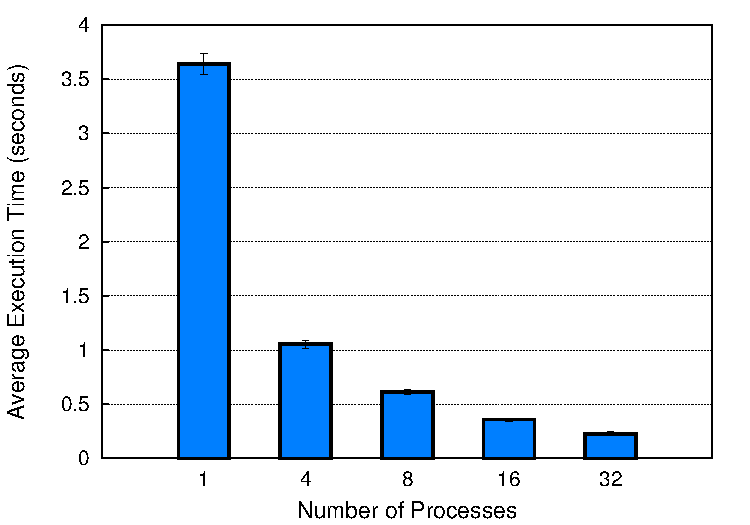
\includegraphics[width=0.65\textwidth]{Figures/MatrixMultiplication.pdf}
	\caption{Εικόνα Παραρτήματος.}
	\label{fig:AppendixFigure}
\end{figure}


% Εκτύπωση του ευρετηρίου (προαιρετικό)
\printindex


% Σελίδες χωρίς αρίθμηση
\pagenumbering{gobble}

\chapter*{\csedimosieuseis}

Προαιρετικά, βάζουμε μία λίστα με τις δημοσιεύσεις του συγγραφέα. % Προαιρετικό

% Σύντομο Βιογραφικό
\chapter*{\cseviografiko}
% Εισαγωγή του κεφάλαιου στα περιεχόμενα
\addstarredchapter{\cseviografiko} % minitoc

Ένα σύντομο βιογραφικό είναι απαραίτητο.

\end{document}
